\documentclass[12pt,a4paper]{report}
\usepackage[utf8]{inputenc}
\usepackage{amsmath}
\usepackage{amsfonts}
\usepackage{amssymb}
\usepackage{graphicx}
\usepackage{color}
\author{Malcolm Watt}

\newcommand{\mat}[1]{\left[ \begin{smallmatrix} #1 \end{smallmatrix} \right]}

\begin{document}
\section*{Chapter 5 Exercises}
\subsection*{Question 5.3}
\textit{(a)} The derivative of $f(x) = x^2 -y$ is $f'(x)=2x$, therefore
the Newton iteration for solving $f(x) = 0$ is $x_{k+1}=x_k - (x_{k}^{2} - y) / 2 x_k$.

\textbf{(b)} The general rule for getting x bits of accuracy given a 4 bit accurate initial guess
is to solve for the number of iterations k in $4 * 2^k = x$. To get 24 bits: $$k = log_2(24 / 4) = 3$$
so we need 3 iterations.

For 53 bits we need $$k = log_2(53/4) = 3.72$$ which rounds up to 4 iterations.

\subsection*{Question 5.4}
We take the given function $$f(x) = x-1-y$$ and take its derivative: $$f'(x) = -x-2.$$
From this, the Newton iteration for solving $f(x) = 0$ is given by
$$x_{k+1} = x_k - (x_k^{-1} - y) / (-x_k^{-2})=x_k + x_k^{2}(x_k^{-1}-y)=2x_k - x_k^{2}y.$$
Since we reduced the terms, there are no divisions in the final formula.

\subsection*{Question 5.6}
\textit{(a)} Since $g'_1(x) = 1- 2x$ and $\vert g'_1(\sqrt{3})\vert = \vert 1 - 2 \sqrt{3} \vert \approx 2.46 > 1$,
the iterative scheme is not convergent.

\textit{(b)} Since $g'_2(x)=1 - 2x / y$ and $ \vert g'_1(\sqrt{3})\vert = \vert 1 - 2\sqrt{3}/3 \vert \approx 0.155 < 1$ so the iterative scheme is locally convergent.

\textit{(c)} $f'(x) = 2x$, so the fixed point iteration function given by Netwon's method is $g(x) = x- (x^2 -y) / 2x$.

\subsection*{Question 5.9}
$x^2_1 - x^2_2 = 0,$ and $2x_1 x_2 = 1$
that is $$f(x) = \left[\begin{smallmatrix}x^2_1 - x^2_2 \\ 2x_1 x_2 - 1 \end{smallmatrix} \right] =
\left[\begin{smallmatrix}0 \\ 0\end{smallmatrix} \right]$$
with starting value $x_0 = \left(\begin{smallmatrix} 0 & 1\end{smallmatrix} \right)^T$.

Our Jacobian is given by $$J_f(x) = \left(\begin{smallmatrix} 2x_1 & -2x_2 \\ 2x_2 & 2x_1 \end{smallmatrix} \right).$$

Since we were given a starting vector of $x_0 = [0, 1]^T$ we have
$$f(x_0) = \left[ \begin{smallmatrix} -1 \\ -1 \end{smallmatrix} \right]$$
and
$$J_f(x_0) = \left[ \begin{smallmatrix} 0 & -2 \\ 2 & 0 \end{smallmatrix} \right]$$

solving the system $$\left[ \begin{smallmatrix} 0 & -2 \\ 2 & 0 \end{smallmatrix} \right] s_0 =
\left[ \begin{smallmatrix} -1 \\ -1 \end{smallmatrix} \right]$$
gives us $$s_0 = \left[ \begin{smallmatrix} -1/2 & 1/2 \end{smallmatrix} \right]^T$$

$$x_1 = x_0 + s_0 = \left[\begin{smallmatrix}0\\1\end{smallmatrix}\right] +
\left[\begin{smallmatrix}0.5\\-0.5\end{smallmatrix}\right] =
\left[\begin{smallmatrix}0.5\\0.5\end{smallmatrix}\right].$$

The result of the first iteration of the Newton method is
$$ x_1 = \left[\begin{smallmatrix}0.5\\0.5\end{smallmatrix}\right].$$

\subsection*{Question 5.10}
If $x_k = x*$ then $f(x_k) = 0$ and

$$x_{k+1} = x_k - f(x_k) \frac{x_k - x_{k-1}}{f(x_k) - f(x_{k-1})} = x* - 0 = x*.$$

If $x_{k-1} = x*$, then $f(x_{k-1}) = f(x*) = 0$ and
$$x_{k+1} = x_k - f(x_k)\frac{x_k - x_{k-1}}{f(x_k) - f(x_{k-1})} = x_k - f(x_k)\frac{x_k - x*}{f(x_k)}
= x_k - (x_k - x*) = x*.$$

in both cases, the next value of x is $x*$.


\section*{Chapter 5 Computer Exercises}
Check the Jupyter notebook! :)
\section*{Chapter 6 Exercises}
\subsection*{Question 6.1}
\textit{(a)} $$f (x) = \frac{1}{2}(x^2_1 - x_2 )^2 + \frac{1}{2}(1 - x_1 )^2 .$$

Both terms are positive, so the smallest value we can hope for is 0. The second
term is zero when $x_1 = 1$, if we hold this then the first term is zero when
$x_2 = 1$. The Function therefore achieves a zero at
$\left[\begin{smallmatrix}x_1\\x_2\end{smallmatrix}\right] = \left[\begin{smallmatrix}1\\1\end{smallmatrix}\right]$.

\textit{(b)} $$x_1 = x_0 - H_f^{-1}(x_k)\Delta f(x_k).$$
$$\Delta f(x) = \left[ \begin{smallmatrix} 2 x_1^3 - 2x_2 x_1 + x_1 - 1\\ -x^2_1 + x_2 \end{smallmatrix}\right] =
\left[ \begin{smallmatrix} 9 \\ -2 \end{smallmatrix}\right]$$
$$H_f(x) = \left[\begin{smallmatrix} 6x_1^2 - 2x_2 + 1 & -2x_1\\
-2x_1 & 1\end{smallmatrix}\right]=
\left[\begin{smallmatrix}
21 & -4\\
-4 & 1\end{smallmatrix}\right]$$

The newton equation to be solved is 
$$\left[\begin{smallmatrix}
21 & -4\\
-4 & 1\end{smallmatrix}\right]s_0 = \left[ \begin{smallmatrix} 9 \\ -2 \end{smallmatrix}\right]
=\left[ \begin{smallmatrix} 0.2 \\ -1.2 \end{smallmatrix}\right]$$

and the next iteration value is $$x_1 = x_0 + s_0 =
\left[ \begin{smallmatrix} 2 \\ 2 \end{smallmatrix}\right] + 
\left[ \begin{smallmatrix} 0.2 \\ -1.2 \end{smallmatrix}\right]=
\left[ \begin{smallmatrix} 2.2 \\ 0.8 \end{smallmatrix}\right]$$

\textit{(c)} Our result gets much closer to the correct value for the $x_2$ term,
however \textit{(d)} our result gets slightly farther away for the $x_1$ term.

\subsection*{Question 6.2}
The gradient and Hessian are given by:
$$f(x)= \frac{1}{2} * \left[ \begin{smallmatrix}  x_1 * (A_{11}x_1 + A_{12} x_2 + ...) + x_2 * (A_{21} x_1 + A{22} x_2 + ...) + ... + x_i (A{i1} x_1 + ... + A{ii} x_i)
 \end{smallmatrix} \right]$$

$$\Delta f(x)= \frac{1}{2} * \left[ \begin{smallmatrix} A_{11} * (A_{11}x_1 + A_{12} x_2 + ...)
+ A_{21} * x_2 + ... + A_{i1} * x_i\\
A_{22} * (A_{21}x_1 + A_{22} x_2 + ...) + A_{12} * x_1 + ... + A_{i2} * x_i\\
...\\
A_{ii} * (A_{i1}x_1 + A_{i2} x_2 + ...) + A_{1i} * x_1 + ... + A_{i-1, i} * x_{i-1}\\
 \end{smallmatrix} \right]$$
$$=\frac{1}{2} * \left[ \begin{smallmatrix} 
A_{11}^2 x_1 + (A_{11} + 1) * (A_{12} x_2 + A_{1i}  x_i)\\
A_{22}^2 x_2 + (A_{22} + 1) * (A_{21}x_1 + ... + A_{2i}  x_i)\\
...\\
A_{ii}^2 x_i + (A_{ii} + 1) * (A_{i1}x_1 + A_{i2} x_2 + ...)\\
 \end{smallmatrix} \right]$$

{\color{red} Damn, I don't know what to do...
My guess is that the b vector subtracts out the ugly terms.
When we do the hessian we're left with like the diagonal or something.

I don't know what argument to make about what the minimal value should be though,
like should it be when the f(x) = 0? I think I'm just going to skip this question.
}

\subsection*{Question 6.3}
From the discussion in section 6.5, we can see clearly that the Hessian
of the Lagrangian function is $$H_L(x, \lambda) = 
\left[ \begin{smallmatrix} B(x, \lambda) & J_g^T(x)\\J_g(x) & O \end{smallmatrix}\right]
$$
Let's look at the 2x2 case with the Hessian as
$$\left[ \begin{smallmatrix} B & J^T \\ J & 0 \end{smallmatrix} \right]$$

for a vector (x, y) we can set up the following:

$$\left( \begin{smallmatrix} x^T & y^T \end{smallmatrix} \right)
\left( \begin{smallmatrix} B & J^T \\ J & 0 \end{smallmatrix} \right)
\left( \begin{smallmatrix} x\\y \end{smallmatrix} \right)
= x^TBx+ 2y^TJx
$$

If $x=0$ and we pick any value of y, the result equals zero, therefore we pass the test for
a positive definite matrix and the matrix can not be positive definite.

\subsection*{Question 6.4}
There is one at $\mat{0\\0},$ and the on-axis ones are $\mat{1.2\\0}$$ and $$\mat{0\\1.5},$
the other three points are given by the intersections of the three lines,
which occur at $\mat{\frac{18}{17}\\ \frac{12}{17}},$ $\mat{\frac{6}{7}\\ \frac{6}{7}}$
and $\mat{\frac{12}{11}\\ \frac{6}{11}}.$

Of which it is clear that $$\mat{\frac{18}{17}\\ \frac{12}{17}}$$ is dominated by the other
two points. Therefore we have a region with 5 vertices:
$$\mat{0\\0}, \mat{1.2\\0}, \mat{0\\1.5}, \mat{\frac{6}{7}\\ \frac{6}{7}}, \mat{\frac{12}{11}\\ \frac{6}{11}}.$$

Evaluated at each of these points the result is (in the same order):
$$0.0, -3.6, -3.0, -4.28, -4.36$$

Therefore the minimum value occurs at $$\mat{\frac{12}{11}\\ \frac{6}{11}}.$$

The graph is shown in the following figure

\begin{center}
\begin{figure}
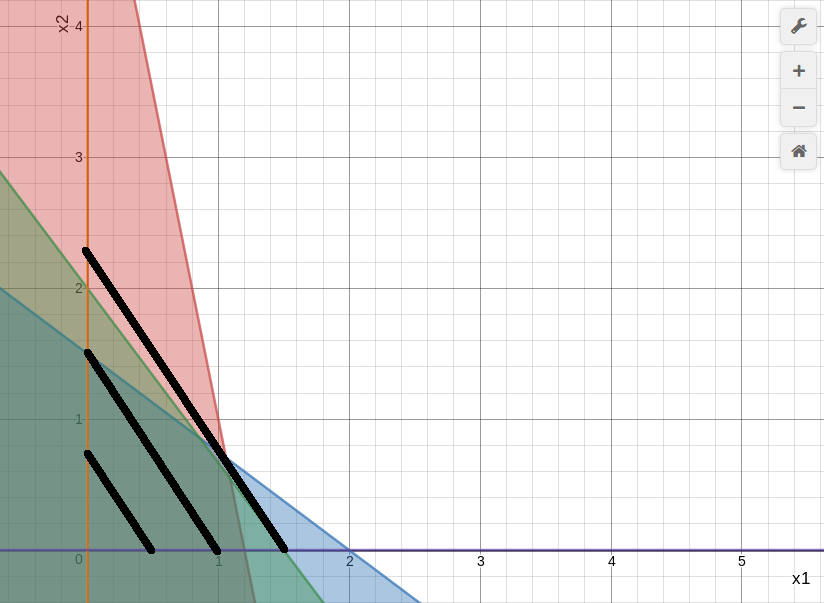
\includegraphics[width=\textwidth]{question64.png} 
\end{figure}
\end{center}

\section*{Chapter 6 Computer Exercises}
Check the Jupyter notebook! :)
\end{document}